\chapter{Fundamentação Teórica}
\label{cap:2fundamentacao}
Neste capítulo o problema inverso será apresentado
em linhas gerais e a inversão sísmica será abordada em maiores detalhes.
Serão apresentados os conceitos relacionados a \textit{Deep Learning}, assim como os
elementos de redes neurais convolucionais. Esta fundamentação
teórica é relevante para o entendimento de como o modelo de rede neural convolucional
pode ser adotado para obter ganho qualitativo e quantitativo no pós-processamento
da inversão sísmica.

\section{Problema Inverso}
A teoria de inversão é utilizada em diversas áreas para inferir os valores de
parâmetros relacionados com processos físicos a partir de um conjunto de dados medidos,
os quais são chamados dados experimentais. É possível descrever o problema inverso
como o processo de obter informações de um sistema parametrizado, a partir de
dados que podem ser medidos por meio de algum experimento físico e das relações teóricas com os parâmetros
desejados, mas que não são passíveis de medição. Frequentemente, algum conhecimento \textit{a priori}
é incorporado ao modelo.

Um sistema físico depende do domínio em estudo. Pode ser uma galáxia para um
astro-físico, pode ser a Terra para um geofísico ou uma partícula quântica
para um físico quântico. Em comum, o fato de que, para ser estudado, um sistema
físico segue três passos básicos: a parametrização do sistema, a modelagem direta e a modelagem inversa \citep{tarantola}.
A parametrização do sistema se refere à definição do conjunto mínimo de elementos (parâmetros)
cujos valores caracterizam completamente o sistema. A escolha dos parâmetros do modelo geralmente
é não única, de modo que dois conjuntos de parâmetros diferentes podem ser equivalentes.

A modelagem direta significa prever os valores dos parâmetros observáveis (dados $d$),
que correspondem a um dado modelo (conjunto de parâmetros $m$). Esta predição pode ser denotada
pela Eq. \ref{eq:frdmdl}. Onde $F(.)$ é chamado operador direto.
\begin{equation}
\label{eq:frdmdl}
d = F(m) 
\end{equation}

Por sua vez, a modelagem inversa se refere ao uso de resultados atuais das medições dos parâmetros
físicos observáveis, para inferir os valores atuais dos parâmetros do modelo (não-observáveis).
O problema inverso pode ser descrito em uma forma discreta como:
\begin{equation}
\label{eq:deqgm}
m = F^{-1}(d)
\end{equation}
onde, $F$ é o sistema físico investigado, e relaciona os parâmetros do modelo $m=(m_1, m_2,...,m_n) \subset R^n$
estimado com os dados observados $d \in R^s$.
Como mencionado no Capítulo \ref{cap:1intro}, um problema inverso possui múltiplas soluções,
de modo que o modelo $m$ pertence a um conjunto de modelos $M$ admissíveis.
Na prática, $d$ pode ser uma função no domínio do tempo e/ou espaço, ou pode ser
uma coleção de observações discretas.

\section{Inversão Sísmica}
Os métodos geofísicos frequentemente envolvem a solução e avaliação de problemas inversos,
pois permitem inferir a distribuição das propriedades físicas na subsuperfície da Terra
usando observações a partir da superfície. A inversão sísmica tem um papel fundamental na solução 
de problemas geofísicos, em especial na caracterização de reservatórios \citep{Bosch2010,Srivastava2009}.
Do ponto de vista prático, as soluções para o problema de inversão sísmica melhoram a exploração e
o gerenciamento na indústria petrolífera, uma vez que os dados sísmicos estimados possuem forte correlação com as
propriedades petrofísicas (porosidade, densidade, etc.) das rochas da subsuperfície \citep{Figueiredo2014}.
Para facilitar o entendimento da inversão sísmica, considere a subsuperfície como sendo formada por camadas
sobrepostas de diferentes tipos de rochas. As regiões onde ocorrem as transições entre tipos
diferentes de rochas são chamadas de \textit{facies} e possuem espessuras diferentes.

\subsection{Aquisição Sísmica}
O dado sísmico é o principal parâmetro observável utilizado na inversão sísmica.
A aquisição destes dados se dá por meio da sísmica de reflexão. Este
método utiliza pulsos sísmicos de uma fonte artificial controlada e monitora a resposta em
função do tempo. Neste sistema, cada região de contato entre dois tipos de rochas
diferentes gera reflexão e refração do pulso sísmico, como demonstrado na Figura
\ref{fig:1sismica}.
De um ponto de vista bastante elementar, é possível intuir que a parte refletida da onda se
propaga em todas as direções, de modo que os componentes horizontal e vertical podem ser medidos.
O componente horizontal (\textit{s-wave}), referente à reflexão horizontal
da onda, é utilizado no processo de inversão conhecido como inversão elástica. Por outro lado, o componente
vertical da onda (\textit{p-wave}), referente à reflexão vertical do pulso emitido, é utilizado no processo
conhecido como inversão acústica.
\begin{figure}[ht!]
\begin{center}
  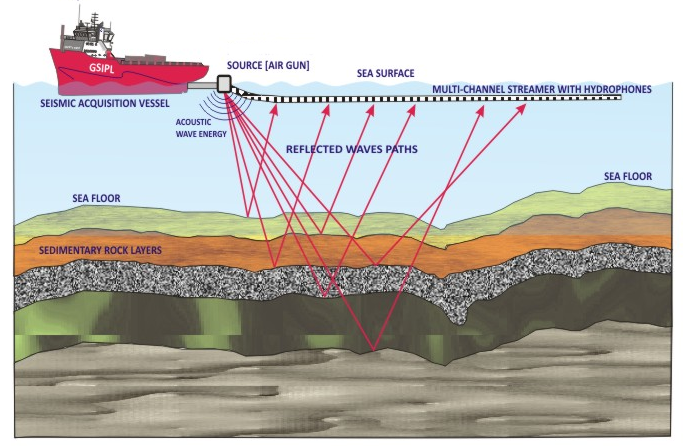
\includegraphics[width=0.8\textwidth]{fig/seismic_survey_2}
  \caption{Método de sísmica de reflexão \citep{figsismica}}
  \label{fig:1sismica}
\end{center}
\end{figure}

O pulso de onda emitido durante a aquisição possui um formato próprio, uma identidade, 
conhecido como \textit{wavelet}. Assim, a resposta sísmica medida
é composta em parte por esta identidade e, em parte, pela característica da interface
entre duas camadas de rochas diferentes, na qual o pulso reflete.
Esta característica é chamada de coeficiente de refletividade (Equação \ref{eq:refletv}):
\begin{equation}
r(t) = \frac{z(t+\delta t)-z(t)}{z(t+\delta t)+z(t)}
\label{eq:refletv}
\end{equation}
onde, $z(t)$ é a impedância acústica no tempo $t$ definida por
$z(t)=\rho(t)v(t)$, onde $\rho(t)$ é a densidade da rocha e $v(t)$ a
velocidade de propagação da onda acústica.
O dado sísmico utilizado na inversão acústica, portanto,
é uma aproximação da resposta da camada terrestre. Pode ainda ser definido como
a convolução entre a \textit{wavelet} de aquisição e o valor de refletividade entre as
camadas, com ângulo de incidência e reflexão de $90^\circ$,
respectivamente. Por este motivo, este modelo é chamado convolucional.
Com os coeficientes de reflexão e a discretização da medida de tempo, é possível
modelar o dado sísmico $d(t)$ aplicando a convolução $*$
da \textit{wavelet} $s$ com os coeficientes de refletividade $r$:
\begin{equation}
d(t) = s(\tau) * \sum_{j-1}^{N}{r(t- t_j) \delta(t - t_j) + e_d(t)}
\end{equation}
onde $N$ é o número total de camadas, $e_d(t)$ representa o ruído aleatório em função do tempo
e cada $d_{xy}$ é chamado de traço sísmico. Um conjunto de traços
sísmicos também é chamado de imagem, seção ou cubo, no caso de um
levantamento 3-D. A \textit{wavelet} ideal seria um pulso tipo delta contendo
todas as frequências, entretanto, na prática as
\textit{wavelets} são pulsos de banda limitada entre $6Hz$ e $65Hz$, o que
limita a frequência da sísmica e sua resolução \citep[p. 11]{sen_livro}.
Como consequência, as imagens resultantes do processo de inversão também terão
o seu espectro de frequência limitado. A Figura \ref{fig:wavelet} ilustra uma
\textit{wavelet} típica extraída de dados reais.
\begin{figure}[htp]
\begin{center}
  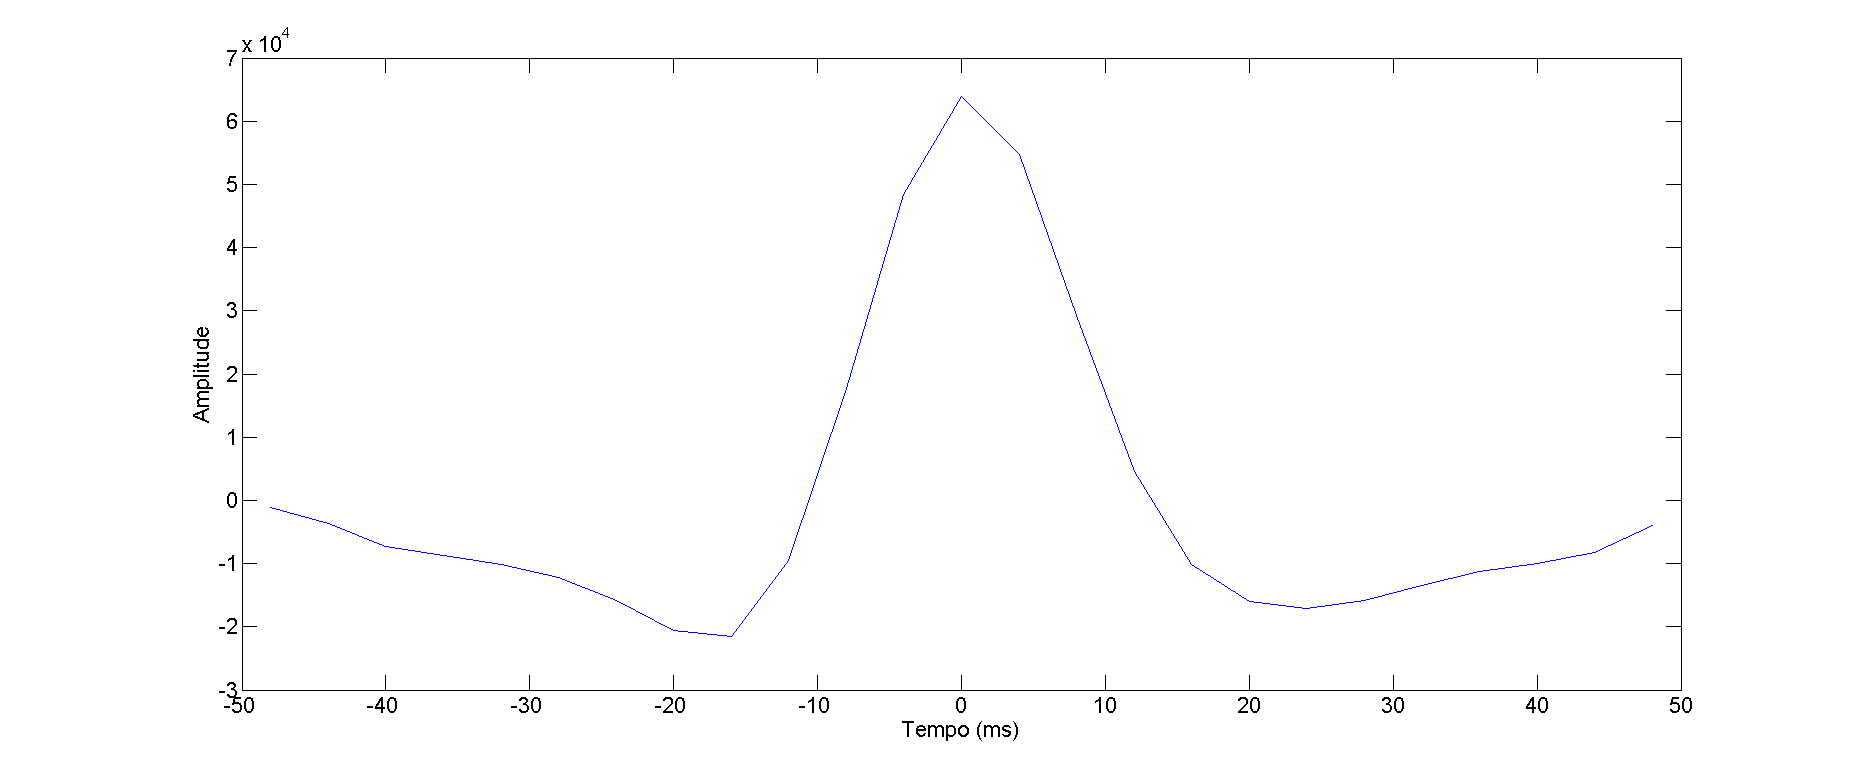
\includegraphics[width=0.8\textwidth]{fig/wavelet}
  \caption{\textit{Wavelet} extraída de dados reais}
  \label{fig:wavelet}
\end{center}
\end{figure}

\section{Redes Neurais Convolucionais}
As Redes Neurais Convolucionais (RNC), também chamadas de redes convolucionais,
são um tipo de rede neural especializada em processamento de dados que possuem uma
topologia conhecida e em forma de grade \citep{Gdfl16}. Exemplos deste tipo de dado são as séries
temporais, que podem ser vistas como uma grade em uma dimensão (1-D) com amostras
em intervalos regulares de tempo, e dados de imagem, que podem ser vistos como
uma grade (2-D) de \textit{pixels}. Este modelo de rede neural é chamado convolucional,
pois emprega a operação de convolução no lugar de multiplicação comum entre matrizes,
em pelo menos uma de suas camadas.

\subsection{Convolução}
A operação de convolução é definida como a integral do produto de duas funções após uma delas sofrer um
certo deslocamento. Considere o exemplo em que se deseja rastrear a localização de uma
nave espacial com um sensor a laser. O sensor disponibiliza uma saída $x(t)$ referente à posição da nave
no tempo $t$. Ambos, $x$ e $t$, são valores reais, de modo que uma saída diferente pode ser obtida
em qualquer instante de tempo. Considerando que o sensor possui um certo ruído, para realizar uma
estimativa mais precisa da posição da nave é preciso ponderar várias medidas de posição juntas.
Como os valores medidos mais recentemente são mais relevantes, se estima uma função peso
$w(a)$, onde $a$ é o tempo de medição. Se esta média ponderada for aplicada a todos os instantes,
a estimativa de posição da nave será suavizada:

\begin{equation}
 s(t) = \int{x(a) w(t-a)da}.
 \label{eq:1}
\end{equation}

A convolução costuma ser denotada com um asterisco e aplicada com o tempo $t$ discretizado para valores inteiros,
dada da seguinte forma:
\begin{equation}
 s(t) = (x * w)(t) = \sum_{a=-\infty}^{\infty}{x(a)w(t-a)}.
 \label{eq:2}
\end{equation}
No contexto das redes convolucionais, $x$ se refere ao conjunto de imagens de entrada 
e $w$ é denominado \textit{kernel} ou filtros. As imagens de entrada são uma sequência multidimensional 
de dados, enquanto os filtros são uma sequência multidimensional de parâmetros a serem 
otimizados pelo algoritmo de aprendizagem.
Nos casos em que o problema compreende imagens $X$ e filtros $W$ utilizados em duas dimensões 
a convolução ganha o seguinte formato:
\begin{equation}
 S(i,j) = (X*W)(i,j) = \sum_{m}\sum_{n}{X(m,n)W(i-m,j-n)}.
\end{equation}

Nas redes convolucionais há pelo menos duas estruturas básicas, a camada convolucional e a camada de \textit{pooling}.
A arquitetura típica de uma RNC compreende duas camadas convolucionais, cada uma seguida por
uma camada \textit{pooling}, como ilustrado na Figura \ref{fig:cnn_basic_arq}. À medida que as imagens progridem
ao longo da rede, suas dimensões diminuem, entretanto, elas se tornam mais profundas
em termos de hierarquia de conceitos extraídos. No topo da pilha de camadas da rede
se adiciona camadas completamente conectadas, sendo que na última camada ocorre a saída prevista.
Esta estrutura de camadas completamente conectadas é a mesma utilizada nas redes neurais tradicionais
do tipo \textit{feedforward}, nas quais todos os nerônios de uma camada estão conectados a todos os
neurônios da camada seguinte. 
\begin{figure}[htp]
\begin{center}
  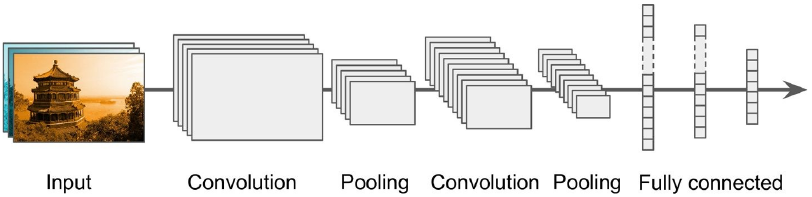
\includegraphics[width=0.8\textwidth]{fig/cnn_basic_arq}
  \caption{Arquitetura típica de uma rede neural convolucional. \citep{aurelien17}}
  \label{fig:cnn_basic_arq}
\end{center}
\end{figure}

A camada convolucional é o elemento mais importante de uma RNC. Esta camada é estruturada
de modo a fazer com que cada um dos seus neurônios esteja conectado a um 
pequeno grupo de \textit{pixels} da camada de entrada (Figura \ref{fig:cnn_arq}) e não a todos os \textit{pixels}, como
ocorre em redes neurais tradicionais. Cada neurônio da camada seguinte se conecta apenas aos neurônios
contidos em uma pequena região da camada anterior e assim sucessivamente. Esta região que define
o grupo de neurônios conectados ao neurônio da próxima camada é chamada \textbf{campo perceptivo}.
Este formato permite o aprendizado de características de baixo nível na primeira camada e de
características de mais alto nível nas camadas seguintes.
\begin{figure}[htp]
\begin{center}
  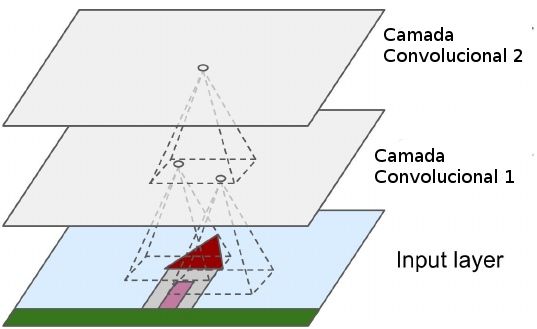
\includegraphics[width=0.6\textwidth]{fig/cnn_arq}
  \caption{Camadas de uma RNC com campos receptivos retangulares.}
  \label{fig:cnn_arq}
\end{center}
\end{figure}

A Figura \ref{fig:cnn_stride} ilustra  um exemplo de campo receptivo e das conexões entre duas camadas em uma rede convolucional.
Considere um neurônio localizado na linha $i$ e coluna $j$ de uma dada camada.
Este neurônio estará conectado às saídas dos neurônios da camada anterior
localizados nas linhas ${i}\times{s_h}$ até ${i}\times{s_h}+f_h - 1$, colunas
${j}\times{s_w}$ até ${j}\times{s_w}+f_w - 1$, onde
$f_h$ e $f_w$ são a altura e a largura do campo receptivo, $s_h$ e $s_w$
são os deslocamentos vertical e horizontal ao longo das imagens da camada anterior.
O tamanho destes deslocamentos é chamado de passo ou \textit{stride}
e quanto maior o \textit{stride}, menor será a imagem resultante na camada seguinte. Para \textit{stride}
de tamanho $0$ a camada seguinte terá as mesmas dimensões da camada anterior.
\begin{figure}[htp]
\begin{center}
  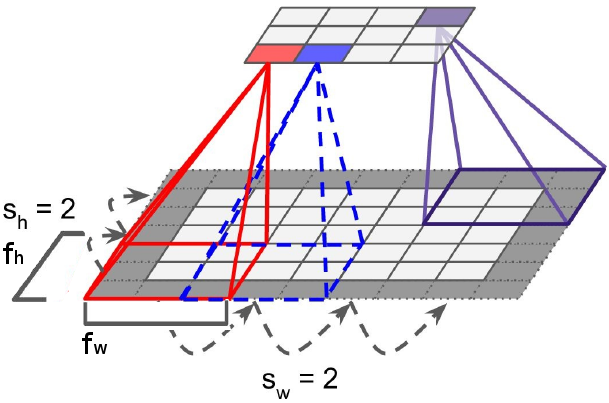
\includegraphics[width=0.6\textwidth]{fig/cnn_layer_stride_2}
  \caption{Conexão entre camadas com campo receptivo 3 x 3 e \textit{strides} de tamanho 2.}
  \label{fig:cnn_stride}
\end{center}
\end{figure}

\subsection{Filtros}
Os filtros (pesos) em uma camada convolucional são representados como uma pequena
imagem com as mesmas dimensões do campo receptivo. São eles os elementos
convolvidos com a imagem de entrada para obter o resultado da camada convolucional.
Durante o treinamento de uma rede convolucional cada elemento dos filtros é otimzado.
A Figura \ref{fig:conv_filt} ilustra dois filtros exemplos e o resolutado da convolução
de cada um com uma certa imagem. O primeiro filtro é um quadrado preto
(\textit{pixels} de valor 0) contendo uma coluna central branca (\textit{pixels} com valor 1). 
Analogamente, o segundo filtro é um quadrado preto contendo uma linha central branca.
É possível notar na imagem da esquerda que as linhas verticais brancas se tornaram mais
evidentes, enquanto as outras partes da imagem se tornaram mais borradas. Na imagem da direita 
a convolução com o filtro horizontal destacou as linhas brancas horizontais, ao passo que
o restante ficou borrado. Assim, quando uma característica é detectada por um neurônio, ela representa
o tipo de padrão da entrada que causará a sua ativação.
Estes padrões podem ser bordas, contornos ou estruturas com outras formas.
\begin{figure}[htp]
\begin{center}
  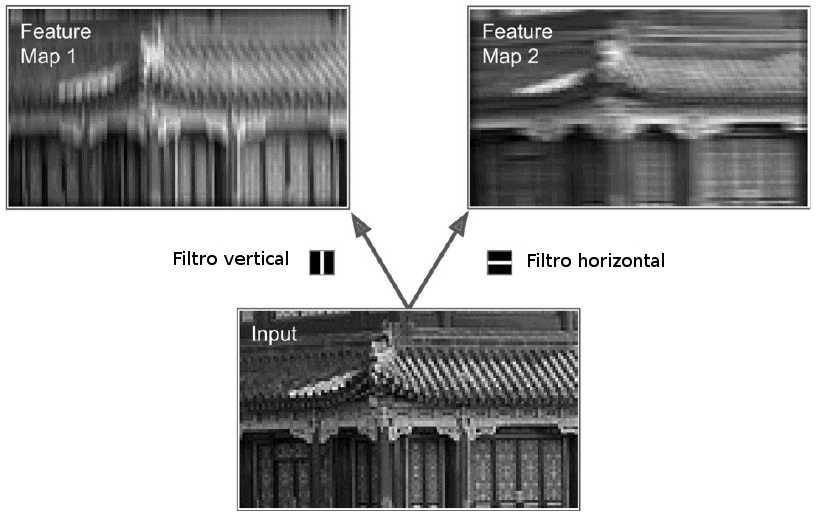
\includegraphics[width=0.7\textwidth]{fig/conv_filt}
  \caption{Aplicação de dois filtros diferentes para obter mapas de características.}
  \label{fig:conv_filt}
\end{center}
\end{figure}

Em situações reais, a camada convolucional possui muitos mapas de características, resultando
em uma representação em 3-D como ilustrado na Figura \ref{fig:featmaps}. Os mapas de características
de uma camada convolucional são o resultado da convolução de uma das imagens de entrada com os diversos
filtros específicos desta camada, de modo que, é possível imaginar que à medida que o número de imagens aumenta,
a estrutura ilustrada se replica horizontalmente.
\begin{figure}[htp]
\begin{center}
  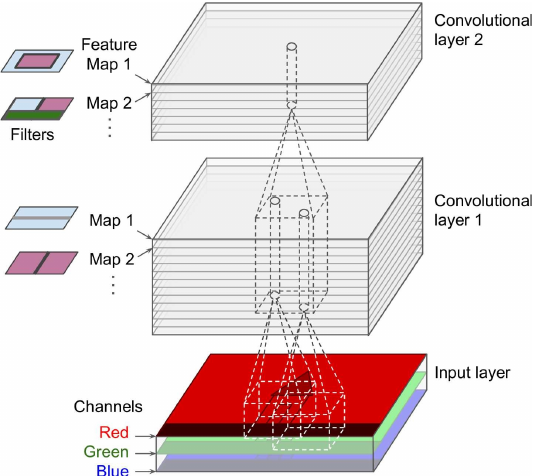
\includegraphics[width=0.6\textwidth]{fig/feat_maps}
  \caption{Camadas convolucionais com múltiplos mapas de características e imagens com três canais.}
  \label{fig:featmaps}
\end{center}
\end{figure}

\subsection{Pooling}
O processamento ao longo de uma rede convolucional ocorre em três estágios. No primeiro estágio
acontecem as convoluções entre as imagens e os filtros, para produzir um conjunto de ativações lineares.
O segundo estágio é chamado estágio de detecção, na qual cada ativação é submetida a uma
função não-linear. O terceiro estágio é chamado de \textit{pooling}, responsável por
modificar a saída da camada convolucional para obter um sumário estatístico das saídas da convolução.
Semelhante ao que ocorre na convolução, a região sobre a qual se aplica o \textit{pooling} é definida por um
campo receptivo e o deslocamento é definido por um \textit{stride}. O \textit{pooling} permite tornar
invariante pequenas translações no conjunto de entrada, ou seja, ainda que haja pequenas translações na
entrada, os valores da maioria das saídas após o \textit{pooling} permanecem iguais.
A Figura \ref{fig:pool} ilustra o funcionamento da função de \textit{pooling} máximo, na qual
o máximo valor de ativação dentro de uma vizinhança é selecionado. Outras funções de \textit{pooling} incluem o valor médio
dentro de uma região retangular, a normalização $L2$ de uma vizinhança, ou a média ponderada baseada na distância do \textit{pixel} central.
\begin{figure}[htp]
\begin{center}
  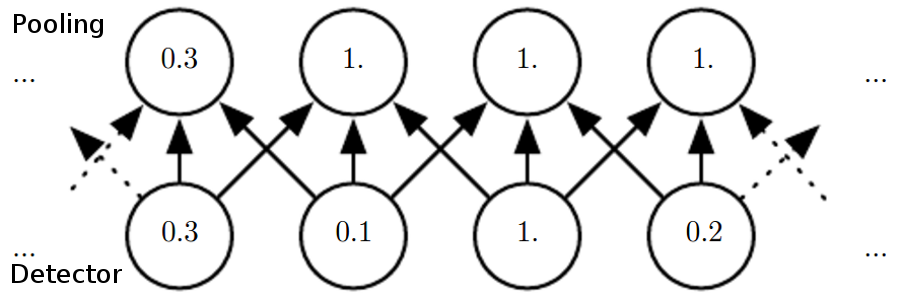
\includegraphics[width=0.7\textwidth]{fig/pool}
  \caption{Operação de \textit{pooling} com campo receptivo de tamanho $3$. Nesta operação é selecionado o máximo valor de ativação da etapa de detecção.}
  \label{fig:pool}
\end{center}
\end{figure}

A propriedade de invariância é útil quando a existência de uma característica é mais relevante que
o local exato onde ela ocorre. Por exemplo, para determinar se o rosto de uma pessoa ocorre em uma certa imagem, não é necessário saber
com precisão o local dos olhos, basta saber se há um olho do lado esquerdo do rosto e outro olho do lado direito
\footnote{O rosto da figura pública Nestor Cerveró, por exemplo, seria facilmente identificável por uma rede convolucional com uma camada de \textit{pooling}}.
Por outro lado, há contextos em que o local da característica é uma informação relevante e deve ser preservada. 
Por exemplo, em modelagem de reservatórios, a detecção de bordas referentes a uma facie selante sobre uma região de reservatório.
Adicionalmente, a operação de \textit{pooling} permite lidar com entradas de tamanho variável. Na classificação de imagens,
as entradas para a camada classificadora devem ter o mesmo tamanho. Assim, o \textit{stride} entre regiões de \textit{pooling} pode variar
para que a camada classificadora receba o mesmo número de sumários estatísticos, independente do tamanho das imagens.

As função de \textit{pooling} sumariza as respostas de vizinhanças separadas por $k$ \textit{pixels}, por isso, o tamanho do seu campo receptivo é menor
que o campo receptivo da convolução. Isto aumenta a eficiência computacional da rede, pois a camada seguinte à de \textit{pooling} terá $k$ vezes
menos entradas para processar. Quando o número de filtros da camada seguinte é função do tamanho da sua entrada, a redução promovida pela
função de \textit{pooling} pode resultar em maior eficiência estatística e redução da quantidade de memória \citep{aurelien17}.

\subsection{Propriedades das Redes Convolucionais}
Por conta da sua arquitetura, as redes convolucionais se sustentam sobre três pilares: interações esparsas, compartilhamentos
de parâmetros e representações equivariantes. As propriedades de interação esparsa e compartilhamento de pesos serão apresentados
em maiores detalhes nesta seção, embora já tenham sido introduzidos de forma intuitiva nas seções anteriores.

As \textbf{interações esparsas}, também chamadas de conectividade esparsa ou pesos esparsos,
ocorre quando os filtros possuem dimensão menor que a entrada, ou seja, a
dimensão do campo receptivo é menor que a dimensão das imagens de entrada.
De um ponto de vista prático, a imagem de entrada pode ter milhares de \textit{pixels}, entretanto, é 
possível detectar apenas pequenas regiões com características de maior relevância na imagem de entrada
com filtros que compreendam apenas algumas dezenas \textit{pixels}.
Por exemplo, é possível identificar características de uma face humana no reconhecimento de pessoas, ou estruturas com
significado geológico em um estudo geofísico. As Figuras \ref{fig:sparse} e \ref{fig:full} ilustram
os modelos de conectividade esparsa e não-esparsa, respectivamente.
É possível notar que na conectividade não-esparsa (Figura \ref{fig:full}) todos os elementos da camada inferior
afetam o elemento em destaque $s_3$ da camada seguinte, enquanto na conectividade esparsa (Figura \ref{fig:sparse}) apenas
três elementos afetam o elemento em destaque. O número de elementos que afetam o elemento em destaque na
conectividade esparsa é definido pelo tamanho do filtro utilizado na convolução.
\begin{figure}[htp]
\begin{subfigure}{.5\textwidth}
  \centering
  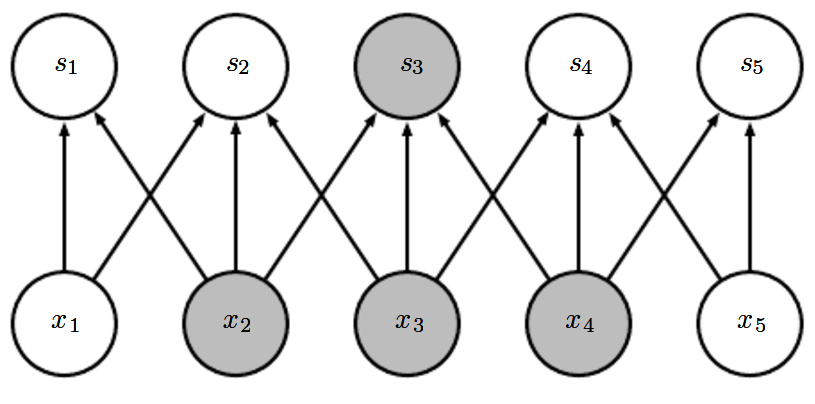
\includegraphics[width=.9\linewidth]{fig/sparse}
  \caption{Conectividade esparsa.}
  \label{fig:sparse}
\end{subfigure}
\begin{subfigure}{.5\textwidth}
  \centering
  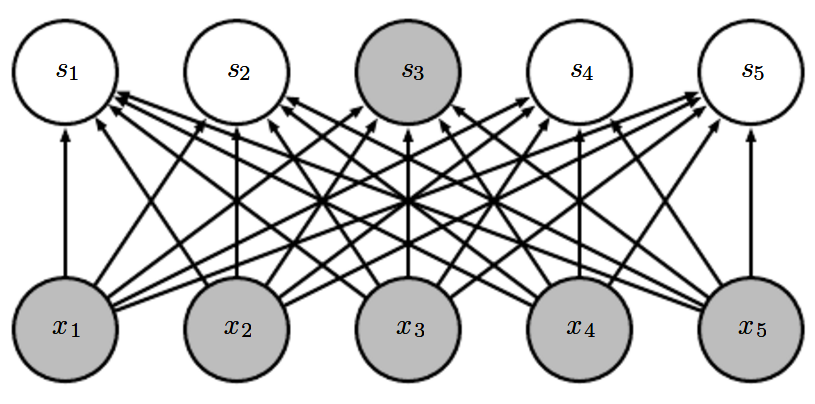
\includegraphics[width=.9\linewidth]{fig/full}
  \caption{Conectividade tradicional.}
  \label{fig:full}
\end{subfigure}%
\end{figure}

O \textbf{compartilhamento de parâmetros}, também chamado de \textbf{pesos amarrados},
se refere ao uso do mesmo parâmetro para mais de uma função no modelo.
Como já mencionado, nas redes neurais tradicionais todos os neurônios de uma camada são conectados a todos os neurônios
da camada anterior e cada neurônio possui um \textit{bias}, como ilustrado na imagem \ref{fig:shallow}.
Entretanto, este modelo é pouco eficiente, pois não tira vantagem da estruturas espaciais das imagens
de entrada \citep{Gdfl16}.
\begin{figure}[htp]
\begin{center}
  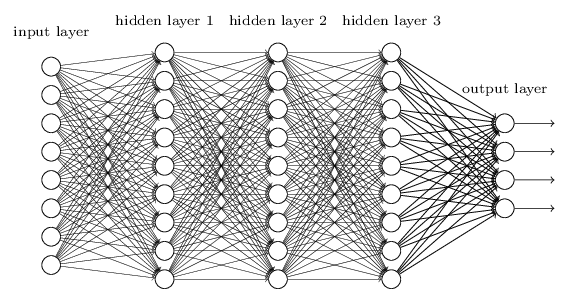
\includegraphics[width=0.7\textwidth]{fig/shallow_nn}
  \caption{Organização de camadas de uma rede neural do tipo \textit{feedforward}.}
  \label{fig:shallow}
\end{center}
\end{figure}
Parece senso comum que estas informações estruturais são muito relevantes em problemas geoestatísticos, afinal as imagens
neste domínio representam estruturas geológicas.

No compartilhamento de pesos a saída de cada neurônio
de uma camada depende apenas do conjunto de neurônios de uma pequena região definida pelo campo receptivo da camada anterior:
\begin{equation}
 {\sigma} \times \bigg( b + \sum_{m}\sum_{n}{w_{m,n}a_{i+m,j+n} \bigg) }
\end{equation}
onde, $\sigma$ é uma função de ativação, $b$ é o valor compartilhado do \textit{bias}, $w_{m,n}$ é
uma matriz de pesos compartilhados (filtros) e $a_{i+m,j+n}$ denota a entrada $a_{x,y}$ na posição
$x,y$. Como o mesmo filtro é convolucionado ao logo da imagem,
os mesmos pesos e \textit{bias} aprendem diferentes características da imagem. Deste modo, cada conjunto de pesos e \textit{bias} é compartilhado
por diferentes regiões em cada imagem e o número de pesos conectados ao neurônio
da camada seguinte diminui em relação ao modelo tradicional. Isto faz com que a convolução seja mais eficiente que a multiplicação de matriz
do ponto de vista de requisitos de memória e eficiência estatística.

O compartilhamento de pesos confere às redes convolucionais a propriedade de \textbf{equivariância} de
translação. Se uma função é equivariante, significa que se a entrada muda,
a saída muda igualmente. Matematicamente, a função $f(x)$ é equivariante à função $g$ se
$f(g(x)) = g(f(x))$. No caso da convolução, se $g$ é uma função que translada a entrada, então
a convolução será equivariante a $g$.
A convolução com imagens cria um mapa 2-D dos locais onde certas características aparecem na entrada.
A propriedade de equivariância permite rastrear objetos transladados na entrada. Se um objeto aparece
em uma determinada posição e, em seguida, aparece em outra posição, sua representação
irá mover a mesma quantidade na saída. É importante frisar que, nas RNC, a propriedade de equivariância
é aplicável apenas para a translação, de modo que a convolução não é equivariante para transformações 
de escala e rotações na imagem.

\section{Resumo}

Este Capítulo detalhou os principais conceitos abordados neste trabalho. O
problema inverso foi introduzido e a inversão sísmica apresentada em
maiores detalhes. Foram apresentados os elementos que compõem as redes
neurais convolucionais: a convolução, as camadas convolucionais, os filtros e a camada de \textit{pooling}.
Foram apresentadas também as propriedades das camadas convolucionais: conectividade esparsa,
compartilhamento de parâmetros e equivariância de translação. O Capítulo seguinte apresenta a
revisão do estado da arte para inversão sísmica e para os modelos de RNC utilizados para Super-resolução.